\documentclass[twocolumn,preprintnumbers,amsmath,amssymb,superscriptaddress,pre]{revtex4}

% paper template
% v20140901

% ams
\usepackage{amsmath,amsfonts,amsthm,amssymb}



% figure
\usepackage{graphicx,epstopdf}
\usepackage{subfigure}
\usepackage{wrapfig}
\usepackage{tabularx}
\usepackage{graphics}

%
\usepackage{enumitem}
\usepackage{color}
\usepackage{adjustbox}

\usepackage{hyperref}

% code listing
\usepackage{listings}             % Include the listings-package
\definecolor{mygreen}{rgb}{0,0.6,0}
\definecolor{mygray}{rgb}{0.5,0.5,0.5}
\definecolor{mymauve}{rgb}{0.58,0,0.82}
\definecolor{hbbgColor}{rgb}{0.98,0.98,0.98}

\lstset{ %
  backgroundcolor=\color{hbbgColor},   % choose the background color; you must add \usepackage{color} or \usepackage{xcolor}
%  basicstyle=\tiny, % the size of the fonts that are used for the code
  basicstyle=\tiny\ttfamily, % the size of the fonts that are used for the code
%  basicstyle=\scriptsize\ttfamily, % the size of the fonts that are used for the code
%  basicstyle=\footnotesize\ttfamily, % the size of the fonts that are used for the code
  breakatwhitespace=false,         % sets if automatic breaks should only happen at whitespace
  breaklines=true,                 % sets automatic line breaking
  captionpos=b,                    % sets the caption-position to bottom
  commentstyle=\color{mygreen},    % comment style
  deletekeywords={...},            % if you want to delete keywords from the given language
  escapeinside={\%*}{*)},          % if you want to add LaTeX within your code
  extendedchars=true,              % lets you use non-ASCII characters; for 8-bits encodings only, does not work with UTF-8
  frame=single,                    % adds a frame around the code
  keepspaces=true,                 % keeps spaces in text, useful for keeping indentation of code (possibly needs columns=flexible)
  keywordstyle=\color{blue},       % keyword style
  language=Sh,                     % the language of the code
  morekeywords={*,...},            % if you want to add more keywords to the set
  numbers=left,                    % where to put the line-numbers; possible values are (none, left, right)
  numbersep=5pt,                   % how far the line-numbers are from the code
  numberstyle=\tiny\color{mygray}, % the style that is used for the line-numbers
  rulecolor=\color{black},         % if not set, the frame-color may be changed on line-breaks within not-black text (e.g. comments (green here))
  showspaces=false,                % show spaces everywhere adding particular underscores; it overrides 'showstringspaces'
  showstringspaces=false,          % underline spaces within strings only
  showtabs=false,                  % show tabs within strings adding particular underscores
  stepnumber=2,                    % the step between two line-numbers. If it's 1, each line will be numbered
  stringstyle=\color{mymauve},     % string literal style
  tabsize=1,                       % sets default tabsize to 2 spaces
  title=\lstname                   % show the filename of files included with \lstinputlisting; also try caption instead of title
}
\lstset{basicstyle=\ttfamily}




% ===============================================================================

% ======= Paper specific ===============
\newcommand{\hbAverage}[1]{\overline{#1}}
\newcommand{\mac}{Mac} 
\newcommand{\hSoX}{\mathbb{X}} % generic set
\newcommand{\hSoN}{\mathbb{N}} % the set of natural numbers
\newcommand{\hSoR}{\mathbb{R}} % the set of real numbers
% ======= Paper specific ===============



% ======= math environment ===============
\theoremstyle{plain}% default
\newtheorem{thm}{Theorem}[section]
\newtheorem{lem}[thm]{Lemma}
\newtheorem{prop}[thm]{Proposition}
\newtheorem*{cor}{Corollary}
\theoremstyle{definition}
\newtheorem{defn}{Definition}[section]
\newtheorem{conj}{Conjecture}[section]
\newtheorem{exmp}{Example}[section]
\theoremstyle{remark}
\newtheorem*{rem}{Remark}
\newtheorem*{note}{Note}

% ======= code ===============
\newcommand{\gitignore}{\hCode{\hCodeDot gitignore}}	% shorten space after dot
\newcommand{\hCodeDot}{{\LARGE .}}					% make dot visible 
\newcommand{\hCode}[1]{{\small \texttt{#1}\,}}		% code
% ======= math ===============
\newcommand{\hProb}[1]{\matbb{P}(#1)} % probability of
\newcommand{\hExpect}[1]{< {#1} >} % expected value of
%
\newcommand{\bugun}{--Draft 25.09.2013--} % version

% ======= reference HB ===============
\newcommand{\reffig}[1]{Fig.~\ref{#1}}    % figure
\newcommand{\refeq}[1]{Eq.~\ref{#1}}      % equation
\newcommand{\reftbl}[1]{Table~\ref{#1}}   % table
\newcommand{\refsec}[1]{Sec.~\ref{#1}}    % section
\newcommand{\reflst}[1]{List.~\ref{#1}}  % listing
% ======= reference HB ===============

% ===============================================================================








% ===============================================================================
\begin{document}

\title{CMPE561 \\ 
Natural Language Processing Course \\
An HMM POS Tagger Implementation with Viterbi Decoding
}
\author{Samet Atdag}
\affiliation{Department of Computer Engineering, Bogazici University, Istanbul}
\date{\today}

% ===============================================================================
\begin{abstract}
	In this homework, an HMM Part-of-Speech Tagger with Viterbi decoding is implemented to detect
	the POS tags of a given text. turkish\_metu\_sabanci\_*.conll dataset is used for training and validation.
	The performance of the tagger is calculated using overall accuracy. A confusion matrix for different types
	of tags (cpostag, postag) is given. 
	\\
	
	The code of the project is in Github account: 
	\href{https://github.com/sametatdag/CMPE561}{https://github.com/sametatdag/CMPE561}.
\end{abstract}


\maketitle
\tableofcontents



% ===============================================================================
\section{Introduction}
\label{sec:intro}
In corpus linguistics, part-of-speech tagging is the process of tagging a word according to it's duty in terms of 
its definition and its context. Context is usually defined as its relationship with adjacent and related words in a
phrase, sentence or paragraph. Hidden Markov Models provides a large series of opportunities for detection
of hidden relationships within a series of information. So that, HMM for POS tagging is used very commonly.

In this study, an HMM POS tagger with Viterbi Decoding is implemented to detect the POS tags of a given text. 
The purpose is building and training an HMM to predict the POS tags of the test input file with a certain performance.


\section{Dataset} 
\begin{itemize}[itemsep=0mm]

  \item turkish\_metu\_sabanci\_train.conll is used for training. It contains ~5000 manually labeled sentences.
  \item turkish\_metu\_sabanci\_val.conll is used for validation. It contains 300 manually labeled sentences.

\end{itemize}


\iffalse
\pagebreak
\begin{table}
\begin{adjustbox}{totalheight=\textheight-2\baselineskip}
\begin{tabular}{ |l|c|c|c|c } 
 \hline
Author & \# of files & \# of training files & \# of test files \\
 \hline
  \hline
abbasGuclu & 15 & 9 & 6 \\
abdullahAymaz & 10 & 6 & 4 \\
ahmetAltan & 10 & 6 & 4 \\
ahmetHakan & 15 & 9 & 6 \\
aliBulac & 10 & 6 & 4 \\
atillaDorsay & 15 & 9 & 6 \\
ayseArman & 15 & 9 & 6 \\
balcicekPamir & 30 & 18 & 12 \\
bekirCoskun & 10 & 6 & 4 \\
bulentKorucu & 10 & 6 & 4 \\
canDundar & 10 & 6 & 4 \\
cemilErtem & 10 & 6 & 4 \\
cemSuer & 10 & 6 & 4 \\
cengizCandar & 10 & 6 & 4 \\
cetinAltan & 30 & 18 & 12 \\
deryaSazak & 10 & 6 & 4 \\
doganHizlan & 15 & 9 & 6 \\
eceTemelkuran & 10 & 6 & 4 \\
ekremDumanli & 30 & 18 & 12 \\
elifSafak & 10 & 6 & 4 \\
emreAkoz & 30 & 18 & 12 \\
emreKongar & 15 & 9 & 6 \\
ergunBabahan & 10 & 6 & 4 \\
ertugrulOzkok & 10 & 6 & 4 \\
fatihAltayli & 30 & 18 & 12 \\
fehmiKoru & 10 & 6 & 4 \\
fikretBila & 10 & 6 & 4 \\
fundaOzkan & 10 & 6 & 4 \\
gulseBirsel & 10 & 6 & 4 \\
guneriCivaoglu & 10 & 6 & 4 \\
hakkiDevrim & 15 & 9 & 6 \\
hasanCemal & 10 & 6 & 4 \\
hasanPulur & 10 & 6 & 4 \\
hasmetBabaoglu & 10 & 6 & 4 \\
hekimogluIsmail & 10 & 6 & 4 \\
hincalUluc & 10 & 6 & 4 \\
huseyinGulerce & 10 & 6 & 4 \\
ismetBerkan & 10 & 6 & 4 \\
mahfiEgilmez & 15 & 9 & 6 \\
mehmetaliBirand & 10 & 6 & 4 \\
mehmetBarlas & 30 & 18 & 12 \\
mehmetOz & 15 & 9 & 6 \\
mehmetTezkan & 10 & 6 & 4 \\
melihAsik & 10 & 6 & 4 \\
mumtazerTurkone & 10 & 6 & 4 \\
muratBardakci & 10 & 6 & 4 \\
muratBelge & 10 & 6 & 4 \\
muratYetkin & 10 & 6 & 4 \\
nazliIlicak & 10 & 6 & 4 \\
nihalKaraca & 10 & 6 & 4 \\
nurayMert & 10 & 6 & 4 \\
omerUrundul & 10 & 6 & 4 \\
oralCalislar & 10 & 6 & 4 \\
raufTamer & 10 & 6 & 4 \\
rehaMuhtar & 10 & 6 & 4 \\
ridvanDilmen & 15 & 9 & 6 \\
ruhatMengi & 15 & 9 & 6 \\
samikohen & 30 & 18 & 12 \\
savasAy & 10 & 6 & 4 \\
serpilYilmaz & 10 & 6 & 4 \\
tahaAkyol & 30 & 18 & 12 \\
tamerKorkmaz & 10 & 6 & 4 \\
tarhanErdem & 10 & 6 & 4 \\
umurTalu & 10 & 6 & 4 \\
yaseminCongar & 10 & 6 & 4 \\
yigitBulut & 10 & 6 & 4 \\
yilmazOzdil & 10 & 6 & 4 \\
yukselAytug & 15 & 9 & 6 \\
zekiCol & 10 & 6 & 4 \\
 \hline
\end{tabular}
\end{adjustbox}
\caption{Properties of 69 Authors dataset, training set and test sets.}
\label{table:1}
\end{table}
% ===============================================================================
\fi

\iffalse
\begin{figure}[h]
\caption{Fig.I. Punctuation characters in the string.punctuation built-in.}
\centering
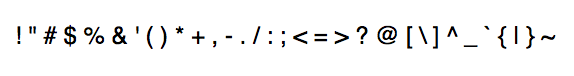
\includegraphics[width=9cm]{punctuation}
\end{figure}
\fi

\section{Pre-processing and Tokenization}
Since a CONLL input files has a certain structure, no pre-processing was required.
\subsection{Sentence Tokenization}
In CONLL file, sentences are separated from each other with 2 consecutive newline characters. While reading
the file, content is splitted by two newlines to tokenize the sentences.
\subsection{POS Tag Type}
Trainer script accepts the POS Tag type: cpostag or postag. CPOSTAG and POSTAG info in CONLL file lays in
3rd and 4th columns. Trainer script uses the pos tag type which is chosen with the parameter.


 
 \section{HMM POS Tagger with Viterbi Decoding}
In this section, I try to clarify how parts of the project works to detect the POS tags. All the implementation 
 is done from scratch; no ready libraries are used. 
 \subsection{Training the HMM}
 For the model, tag transition probabilities (Fig. 1) and observation likelihoods (Fig. 2) are calculated using bi-gram word counts.
 \begin{figure}[h]
\caption{Tag transition probabilities.}
\centering
\include{?}
graphics[width=4cm]{tagtransition}
\end{figure}

 \begin{figure}[h]
\caption{Word likelihood probabilities.}
\centering
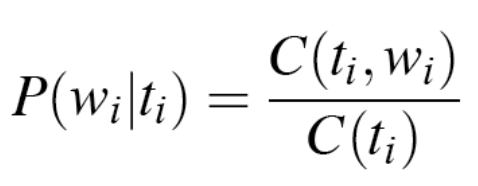
\includegraphics[width=4cm]{wordlikelihood}
\end{figure}

Instead of training the HMM for each run, trained parameters are saved into 2 files when the training script is finished:
 \begin{itemize}[itemsep=0mm]
  \item tag\_transitions.txt : Contains tag transition probabilities in JSON format.
  \item observation\_likelihoods.txt : Contains word likelihoods in JSON format.
\end{itemize} 

 \subsection{Tagging the novel data}
 Tagging is done via running hmm\_tagger.py. This script splits the given text into sentences, decodes the input
 using a Viterbi backtracing matrix and creates an output file. 
 
 Created output file contains 3 column structure:
 WORD  Estimated\_Tag  True\_Tag
 
 \textit{Sidenote}:This structure is slightly different than what is defined in the homework text. Normally, True\_Tag should be 
 in a gold standard file. But since the given test file contains a very tiny dataset (only two sentences), 
 we are advised to use the validation  set for the testing purposes. So that, for the sake of convenience, 
 I put gold standard into this output file.
 
 
  \subsection{Evaluating the results} 
To evaluate the accuracy, we should run evaluate\_hmm\_tagger.py. This file takes the output file which was generated at the 
end of previous step, calculates the accuracy and prints out. 

Also, this script prints out a confusion matrix.
 
 
 
 \iffalse
 \begin{itemize}[itemsep=0mm]
  \item Read all files belonging to the class
  \item Tokenize files
  \item Count the words 
  \item Add word counts to global vocabulary
  \item Add word counts to trained model-class
\end{itemize}
\fi

 \section{Performance Evaluation}
 In this section, the performance of the classifier is given. Overall accuracy for two different POS Tag types (cpostag, postag) 
 is calculated for performance evaluation. Also confusion matrices for them is given.

 \subsection{Accuracy Results}



 \begin{table}[!h]
\begin{tabular}{ |l|c|c|c|  } 
\hline
 & CPOSTAG & POSTAG & Average \\
 \hline
 \hline
Accuracy & 27,011\% & 27,255\% & 27,133\% \\
 \hline
\end{tabular}
\caption{Overall Accuracy for CPOSTAG and POSTAG}
\label{table:1}
\end{table}



\begin{table}[!h]
\scalebox{0.7}{
\begin{tabular}{ |l|c|c|c|c|c|c|c|c|c|c|c|c|c|c|} 
\hline
 & Adv &	Punc &	Noun &	Adj &	Verb &	Det &	Pron &	Postp &	Conj &	Ques &	Num &	Interj &	Dup &	Zero \\
 \hline
 \hline
Adv & 0 &	60 &	86 &	0 &	78 &	0 &	0 &	0 &	0 &	0 &	0 &	0 &	0 &	0 \\
Punc & 300 &	59 &	102 &	0 &	69 &	0 &	0 &	0 &	0 &	0 &	0 &	0 &	0 &	0 \\
Noun & 0 &	460 &	747 &	0 &	491 &	0 &	0 &	0 &	0 &	0 &	0 &	0 &	0 &	0 \\
Adj & 0 &	142 &	173 &	0 &	142 &	0 &	0 &	0 &	0 &	0 &	0 &	0 &	0 &	0 \\
Verb & 0 &	261 &	379 &	3 &	424 &	0 &	0 &	0 &	0 &	0 &	0 &	0 &	0 &	0 \\
Det & 0 &	38 &	71 &	0 &	94 &	0 &	0 &	0 &	0 &	0 &	0 &	0 &	0 &	0 \\
Pron & 0 &	22 &	29 &	0 &	27 &	0 &	0 &	0 &	0 &	0 &	0 &	0 &	0 &	0 \\
Postp & 0 &	24 &	35 &	0 &	20 &	0 &	0 &	0 &	0 &	0 &	0 &	0 &	0 &	0 \\
Conj & 0 &	31 &	58 &	0 &	43 &	0 &	0 &	0 &	0 &	0 &	0 &	0 &	0 &	0 \\
Ques & 0 &	0 &	1 &	0 &	0 &	0 &	0 &	0 &	0 &	0 &	0 &	0 &	0 &	0 \\
Num & 0 &	8 &	23 &	0 &	11 &	0 &	0 &	0 &	0 &	0 &	0 &	0 &	0 &	0 \\
Interj & 0 &	0 &	0 &	0 &	2 &	0 &	0 &	0 &	0 &	0 &	0 &	0 &	0 &	0 \\
Dup & 0 &	0 &	0 &	0 &	0 &	0 &	0 &	0 &	0 &	0 &	0 &	0 &	0 &	0 \\
Zero & 0 &	0 &	0 &	0 &	0 &	0 &	0 &	0 &	0 &	0 &	0 &	0 &	0 &	0 \\
 \hline
\end{tabular}
}
\caption{Confusion matrix for POSTAG type. Rows represent true tags, columns represent estimated tags.}
\label{table:2}
\end{table}


\begin{table}[!h]
\scalebox{0.7}{
\begin{tabular}{ |l|c|c|c|c|c|c|c|c|c|c|c|c|c|c|} 
\hline
 & Adv &	Punc &	Noun &	Adj &	Verb &	Det &	Pron &	Postp &	Conj &	Ques &	Num &	Interj &	Dup &	Zero \\
 \hline
 \hline
Adv &	0 &	0 &	80 &	68 &	76 &	0 &	0 &	0 &	0 &	0 &	0 &	0 &	0 &	0 \\
Punc &	300 &	0 &	77 &	71 &	81 &	1 &	0 &	0 &	0 &	0 &	0 &	0 &	0 &	0 \\
Noun &	0 &	10 &	660 &	472 &	545 &	11 &	0 &	0 &	0 &	0 &	0 &	0 &	0 &	0 \\
Adj &	0 &	2 &	153 &	165 &	136 &	1 &	0 &	0 &	0 &	0 &	0 &	0 &	0 &	0 \\
Verb &	0 &	42 &	383 &	248 &	394 &	0 &	0 &	0 &	0 &	0 &	0 &	0 &	0 &	0 \\
Det &	0 &	0 &	60 &	37 &	106 &	0 &	0 &	0 &	0 &	0 &	0 &	0 &	0 &	0 \\
Pron &	0 &	0 &	29 &	24 &	23 &	2 &	0 &	0 &	0 &	0 &	0 &	0 &	0 &	0 \\
Postp &	0 &	0 &	36 &	24 &	19 &	0 &	0 &	0 &	0 &	0 &	0 &	0 &	0 &	0 \\
Conj &	0 &	0 &	53 &	32 &	47 &	0 &	0 &	0 &	0 &	0 &	0 &	0 &	0 &	0 \\
Ques &	0 &	0 &	0 &	0 &	1 &	0 &	0 &	0 &	0 &	0 &	0 &	0 &	0 &	0 \\
Num &	0 &	0 &	20 &	9 &	13 &	0 &	0 &	0 &	0 &	0 &	0 &	0 &	0 &	0 \\
Interj &	0 &	0 &	0 &	0 &	2 &	0 &	0 &	0 &	0 &	0 &	0 &	0 &	0 &	0 \\
Dup &	0 &	0 &	0 &	0 &	0 &	0 &	0 &	0 &	0 &	0 &	0 &	0 &	0 &	0 \\
Zero &	0 &	0 &	0 &	0 &	0 &	0 &	0 &	0 &	0 &	0 &	0 &	0 &	0 &	0 \\
 \hline
\end{tabular}
}
\caption{Confusion matrix for CPOSTAG type. Rows represent true tags, columns represent estimated tags.}
\label{table:3}
\end{table}
\pagebreak
\hfill





\section{Comments on the Results}
There are two remarkable observations in this experiment. First of all, the overall 
performance is particularly weak for such a task. When I run the same algorithm with another
implementation, it is clearly seen that performance may reach to 60\%. This points to 
a bug or a mis-implementation in the code. 

Secondly, confusion matrices show never used tags in the validation set. When manually 
checked, there is no never-used-tags in the validation set. Again, this points to a mis-implementation.

\section{Notes and Future Work}
It is worth to state that instead of using a gold standard file, I put true tags into evaluation script input
file for convenience. Another mark is that for unknown words, I take probability as 0.0, which leads to 
broken Markov series. 

There are missing points and obvious bugs in the code, but I left them with concerning the tight time schedule.

As for the future work, first step would be the fixing obvious bugs. Then the next step is testing the tagger with a larger 
validation set. A cross validation with another tagger would be a nice playground.

 \section{Conclusion}
To conclude, in this study, I learned how to implement an HMM POS Tagger with Viterbi decoding. 
I evaluated the results using overall accuracy and a confusion matrix. This was a informative study.


\end{document}

I